\documentclass[tikz,border=4pt]{standalone}
\usepackage{amsmath}
\usepackage{amssymb}
\usetikzlibrary{arrows.meta, positioning, fit, backgrounds, calc}

\tikzset{
  basebox/.style={
    draw=black!70,
    fill=black!4,
    rounded corners=3pt,
    align=center,
    font=\small,
    inner sep=6pt,
    minimum height=9mm,
  },
  extbox/.style={
    draw=orange!70!black,
    fill=orange!12,
    line width=0.9pt,
    rounded corners=3pt,
    align=center,
    font=\small,
    inner sep=6pt,
    minimum height=9mm,
  },
  groupbox/.style={
    draw=black!55,
    dashed,
    rounded corners=4pt,
    inner sep=10pt,
    font=\small\bfseries,
  },
  arr/.style={-{Stealth[length=2.2mm]}, semithick, draw=black!65},
  darr/.style={-{Stealth[length=2mm]}, dashed, draw=black!45},
  nlabel/.style={font=\scriptsize, align=center, text=black!75},
}

\begin{document}
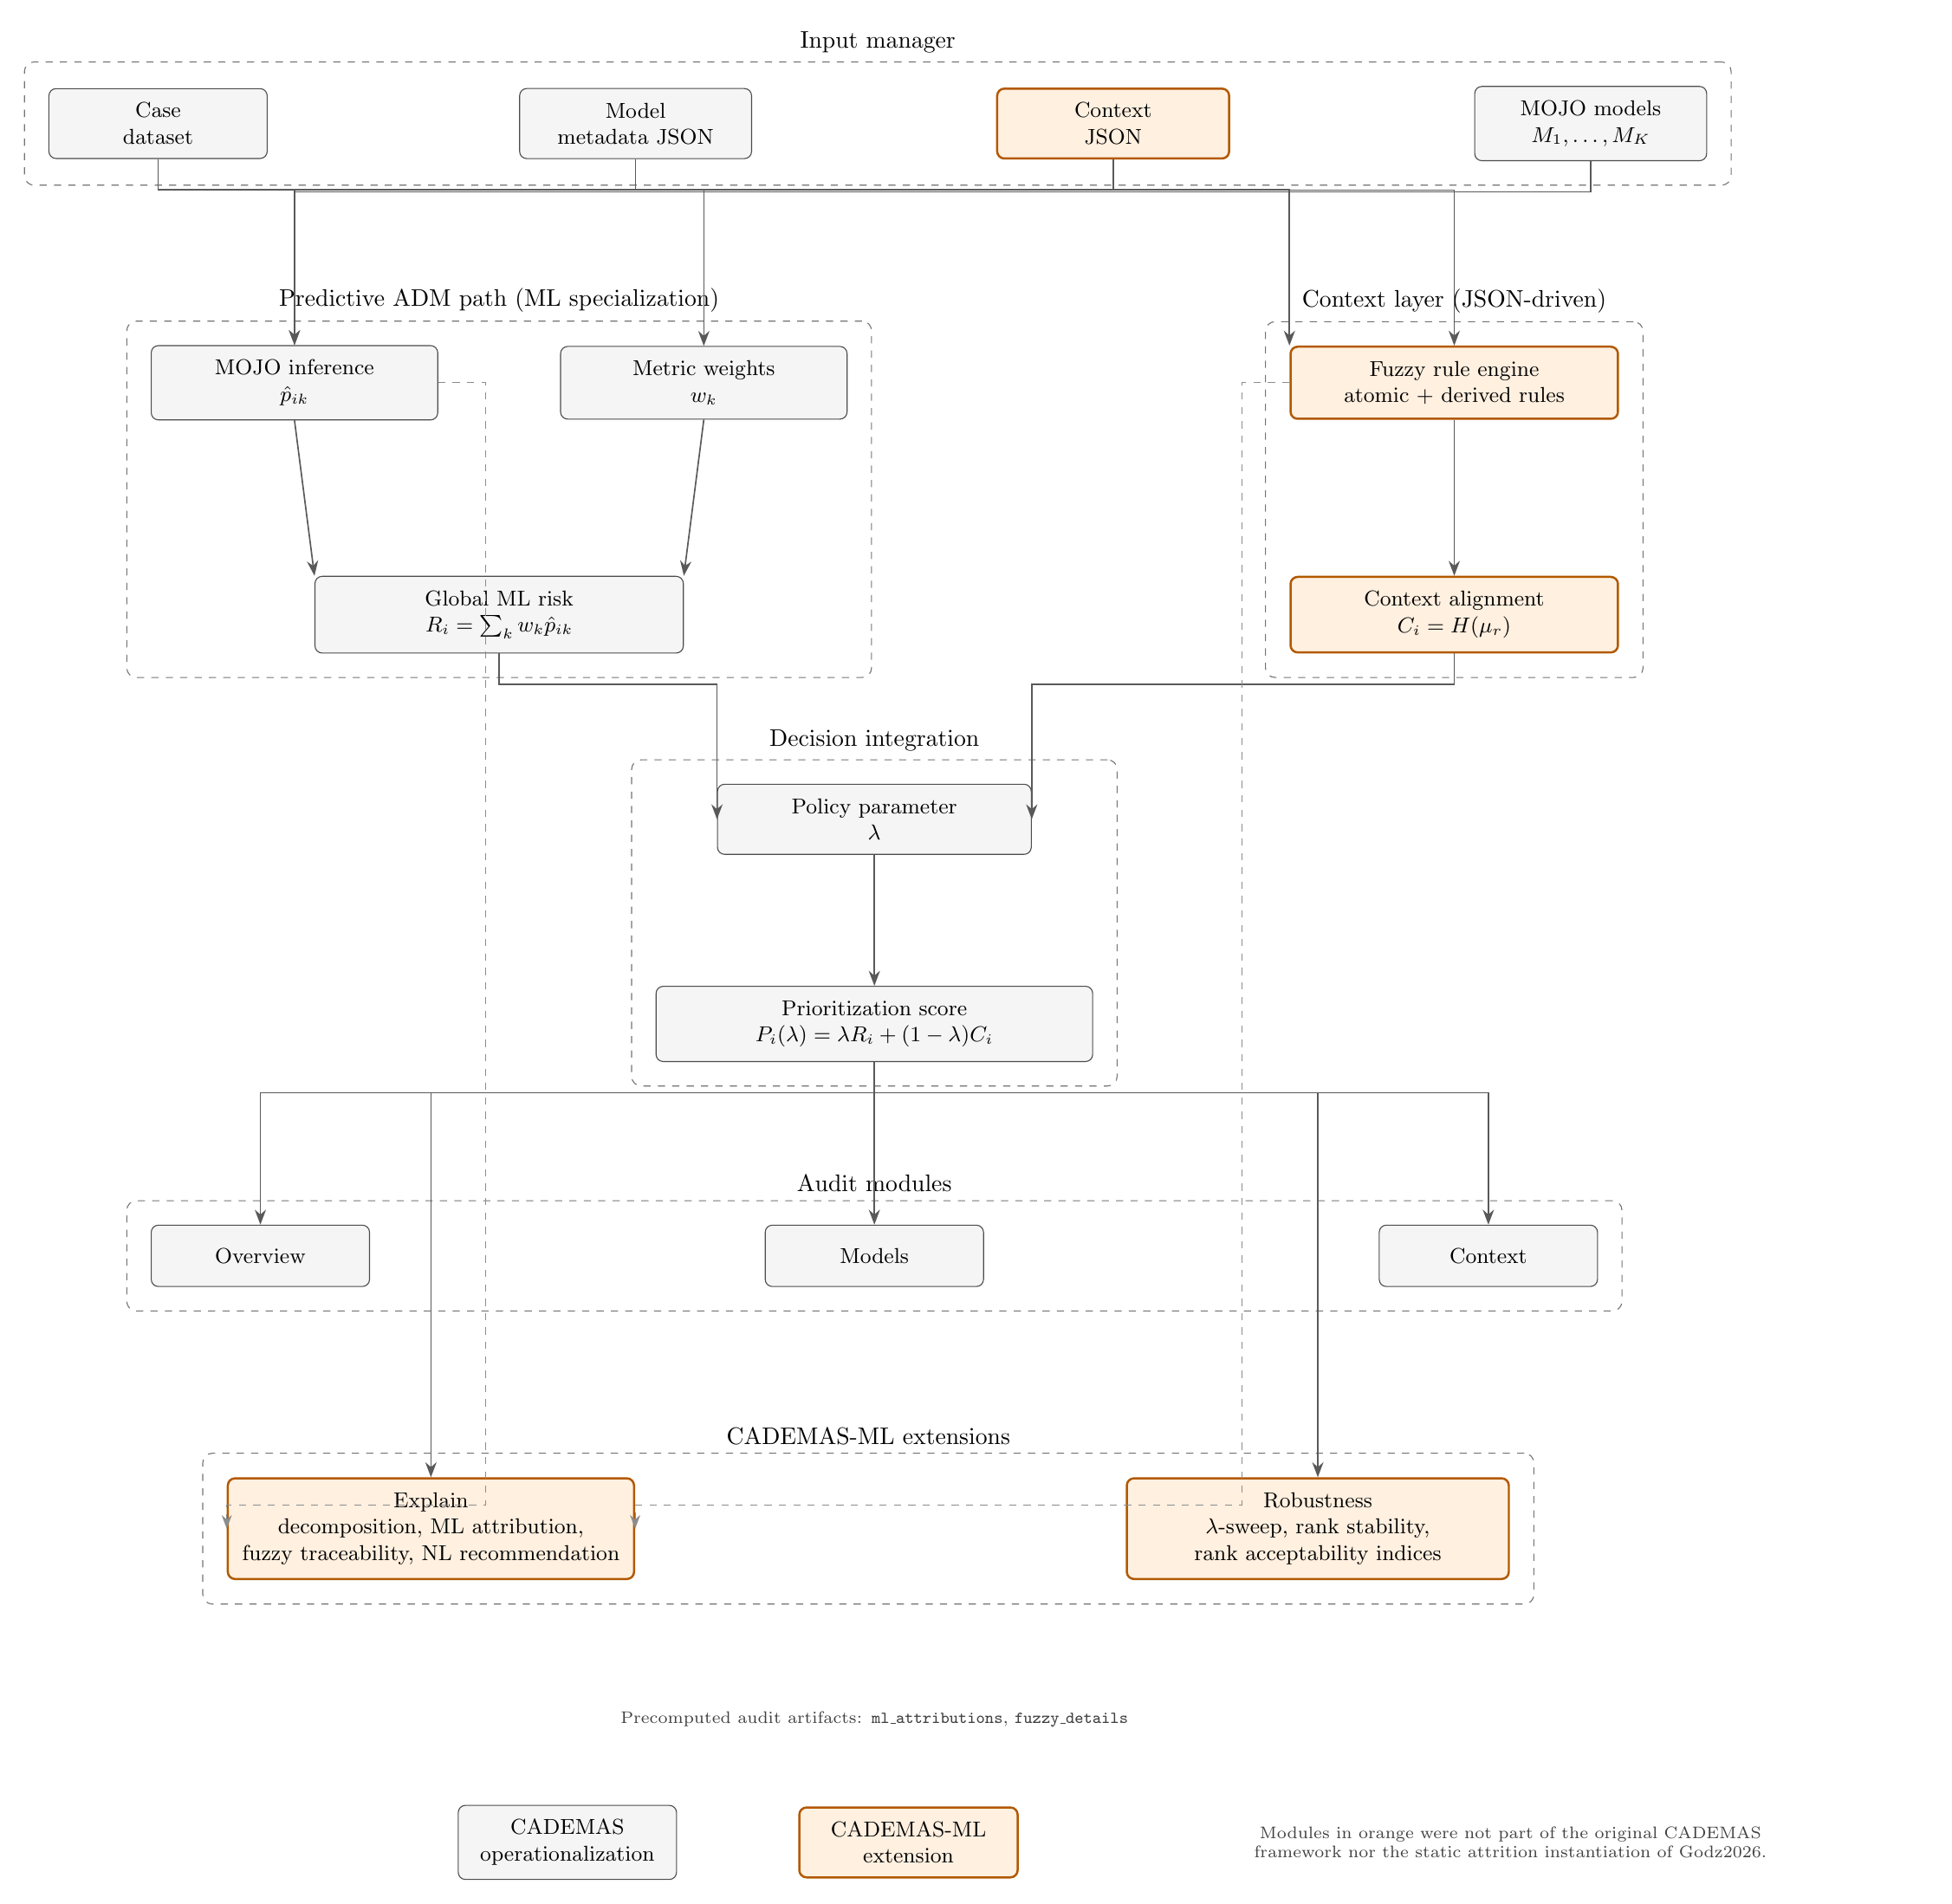
\begin{tikzpicture}[x=1cm, y=1cm]

% --- Input manager (full width) ---
\node[basebox, minimum width=3.2cm] (csv) at (-10.5, 0) {Case\\dataset};
\node[basebox, minimum width=3.4cm] (modeljson) at (-3.5, 0) {Model\\metadata JSON};
\node[extbox, minimum width=3.4cm] (ctxjson) at (3.5, 0) {Context\\JSON};
\node[basebox, minimum width=3.4cm] (mojos) at (10.5, 0) {MOJO models\\$M_1,\ldots,M_K$};

\begin{scope}[on background layer]
  \node[groupbox, fit=(csv) (modeljson) (ctxjson) (mojos), label=above:{Input manager}] (inputlayer) {};
\end{scope}

% --- Predictive path (left column) ---
\node[basebox, minimum width=4.2cm] (infer) at (-8.5, -3.8) {MOJO inference\\$\hat{p}_{ik}$};
\node[basebox, minimum width=4.2cm] (weights) at (-2.5, -3.8) {Metric weights\\$w_k$};
\node[basebox, minimum width=5.4cm] (ri) at (-5.5, -7.2) {Global ML risk\\$R_i=\sum_k w_k\hat{p}_{ik}$};

\begin{scope}[on background layer]
  \node[groupbox, fit=(infer) (weights) (ri), label=above:{Predictive ADM path (ML specialization)}] (mlpath) {};
\end{scope}

% --- Context path (right column) ---
\node[extbox, minimum width=4.8cm] (fuzzy) at (8.5, -3.8) {Fuzzy rule engine\\atomic + derived rules};
\node[extbox, minimum width=4.8cm] (ci) at (8.5, -7.2) {Context alignment\\$C_i=H(\mu_r)$};

\begin{scope}[on background layer]
  \node[groupbox, fit=(fuzzy) (ci), label=above:{Context layer (JSON-driven)}] (ctxpath) {};
\end{scope}

% --- Decision integration (center) ---
\node[basebox, minimum width=4.6cm] (lambda) at (0, -10.2) {Policy parameter\\$\lambda$};
\node[basebox, minimum width=6.4cm] (pi) at (0, -13.2) {Prioritization score\\$P_i(\lambda)=\lambda R_i+(1-\lambda)C_i$};

\begin{scope}[on background layer]
  \node[groupbox, fit=(lambda) (pi), label=above:{Decision integration}] (decision) {};
\end{scope}

% --- Audit modules (spread row) ---
\node[basebox, minimum width=3.2cm] (overview) at (-9, -16.6) {Overview};
\node[basebox, minimum width=3.2cm] (models) at (0, -16.6) {Models};
\node[basebox, minimum width=3.2cm] (context) at (9, -16.6) {Context};

\begin{scope}[on background layer]
  \node[groupbox, fit=(overview) (models) (context), label=above:{Audit modules}] (audit) {};
\end{scope}

% --- CADEMAS-ML extensions (wide row) ---
\node[extbox, minimum width=5.6cm] (explain) at (-6.5, -20.6) {Explain\\decomposition, ML attribution,\\fuzzy traceability, NL recommendation};
\node[extbox, minimum width=5.6cm] (robust) at (6.5, -20.6) {Robustness\\$\lambda$-sweep, rank stability,\\rank acceptability indices};

\begin{scope}[on background layer]
  \node[groupbox, fit=(explain) (robust), label=above:{CADEMAS-ML extensions}] (extensions) {};
\end{scope}

% --- Precomputed artifacts note ---
\node[nlabel, text width=22cm] (cache) at (0, -23.4) {Precomputed audit artifacts: \texttt{ml\_attributions}, \texttt{fuzzy\_details}};

% --- Legend ---
\node[basebox, minimum width=3.2cm] (legbase) at (-4.5, -25.2) {CADEMAS\\operationalization};
\node[extbox, minimum width=3.2cm] (legext) at (0.5, -25.2) {CADEMAS-ML\\extension};
\node[nlabel, text width=12cm, anchor=west] at (3.2, -25.2) {Modules in orange were not part of the original CADEMAS framework nor the static attrition instantiation of Godz2026.};

% --- Arrows: inputs to processing ---
\draw[arr] (mojos.south) -- ++(0,-0.45) -| (infer.north);
\draw[arr] (modeljson.south) -- ++(0,-0.45) -| (infer.north);
\draw[arr] (modeljson.south) -- ++(0,-0.45) -| (weights.north);
\draw[arr] (infer.south) -- (ri.north west);
\draw[arr] (weights.south) -- (ri.north east);

\draw[arr] (csv.south) -- ++(0,-0.45) -| (fuzzy.north west);
\draw[arr] (ctxjson.south) -- ++(0,-0.45) -| (fuzzy.north);
\draw[arr] (fuzzy.south) -- (ci.north);

% --- Arrows: to decision ---
\draw[arr] (ri.south) -- ++(0,-0.45) -| (lambda.west);
\draw[arr] (ci.south) -- ++(0,-0.45) -| (lambda.east);
\draw[arr] (lambda.south) -- (pi.north);

% --- Arrows: to output modules ---
\draw[arr] (pi.south) -- ++(0,-0.45) -| (overview.north);
\draw[arr] (pi.south) -- ++(0,-0.45) -| (models.north);
\draw[arr] (pi.south) -- ++(0,-0.45) -| (context.north);
\draw[arr] (pi.south) -- ++(0,-0.45) -| (explain.north);
\draw[arr] (pi.south) -- ++(0,-0.45) -| (robust.north);

% --- Dashed audit reuse into Explain ---
\draw[darr] (infer.east) -- ++(0.7,0) |- ($(explain.west)+(0,0.35)$) -- (explain.west);
\draw[darr] (fuzzy.west) -- ++(-0.7,0) |- ($(explain.east)+(0,0.35)$) -- (explain.east);

\end{tikzpicture}
\end{document}
